\documentclass[11pt, letterpaper, journal]{IEEEtran}

\usepackage[utf8]{inputenc}
\usepackage[letterpaper, margin=1.5cm]{geometry}
\usepackage{amsmath}
\usepackage{amssymb}
\usepackage{amsthm}
\usepackage[title]{appendix}
\usepackage{authblk}
\usepackage{cite}
\usepackage[font=scriptsize]{caption}
\usepackage{graphicx}
\usepackage{subcaption}
\usepackage{multicol}
\usepackage{lipsum}
\usepackage{subfig}
\usepackage[dvipsnames]{xcolor}
\usepackage{hyperref}

% Some general setting
\graphicspath{ {./statics/} }
\captionsetup{justification=raggedright, singlelinecheck=false}


\title{Project 2: Arctic Cloud Detection}
\author[1]{Devin Ti}
\author[1]{Ryan Tang}
\affil[1]{Duke University, Statistical Science}

\date{December 6th 2022}

\begin{document}
\maketitle

\section{Introduction}
Global warming and how surface air temperatures changes has been a general scientific interest and public policy issue. In addition, many global climate studies predicted the global surface air temperature has the strongest correlation with the increase of the Arctic's atmospheric carbon dioxide level. Hence understanding how carbon dioxide changes in the Arctic is crucial to studying global warming. As the Arctic gets warmer, water vapors and changes in the distribution and proportionality of clouds can lead to further warming and spatial sensitivity, which indicates we need a systematic, accurate way of studying cloud distribution in the Arctic. However, such a study has its unique challenges. Primarily, the current algorithm not being well-suited for distinguishing clouds from ice particles because the two particles are similar in the lens of radiation measurements. MISR data offers a potential solution and introduces a sheer amount of data volume. But the currently deployed algorithm in MISR is not particularly targeted for detecting clouds over bright surfaces in polar regions. At the same time, computational constraints also limit the existing algorithm's performance. Therefore, coming up with a computationally efficient algorithm that delivers accurate detection is of the utmost importance.

MISR provides Arctic satellite images on each orbit on each path every 16 days interval. Each resulting data unit is an image concentrating on a particular, repeating Arctic location patch. Tao and other team members took the time to manually label the data unit with the aid of a labeling algorithm from Jet Propulsion Laboratory, which resulted in 71.5\% of conservative, expert label coverage at the pixel level for evaluating the algorithms. Furthermore, Tao's team introduced ELCM, a cloud detection algorithm based on the three expert-designed features using just if-else hard-coded rules, and utilized Quadratic Discriminant Analysis (QDA) for probabilistic prediction on top of ELCM labels that achieved astonishing results both in terms of precision and recall.

Tao's team introduced three expertly designed features through domain knowledge: CORR, SD, and NDAI. On a high level, these features were constructed through spatial convolution over a small grid under the knowledge that the aggregated radiation from multiple cameras is different between smoothed surfaces, ice and snow, and cloud. We should expect high CORR and small SD over clear or low-altitude cloud areas. NDAI provides a proxy to the visible wavelength where we should expect smaller, less volatile measures for ice and snow-covered surface than low-altitude clouds to further aid in distinguishing between the surface area from the low-altitude cloud.

Despite the amazing work done by Tao's team, constructing the cloud detection algorithm using a few hard-coded linear rules is not ideal. We can certainly do better by introducing a more sophisticated model for predicting cloud presence. Here, by utilizing the expert labels and the engineered features, we tested the performance on a few state-of-art methods and conducted an in-depth modeling calibration analysis for future potential improvements. 

\section{Exploration}
The dataset consists of 3 images shot at the same Arctic location from different orbits. Each consists of $305 \times 382$ pixels that are labeled, \{-1 = Not Cloudy, 0 = Not Sure, 1 = Cloudy\}. The former two categories are pixels that experts annotate, and the latter 'Unlabelled' category is pixels that were not. The labeling process was conservative, so pixels that are not totally obvious are left unlabelled. Along with an X and Y coordinate for each pixel, each pixel is associated with 8 covariates. In this section, we conduct initial exploratory data analysis, which greatly influenced our later modeling choices and testing-validation strategies.

\subsection{Label Dispersion}
\begin{figure*}[!h]
\centering
% \captionsetup{justification=centering}
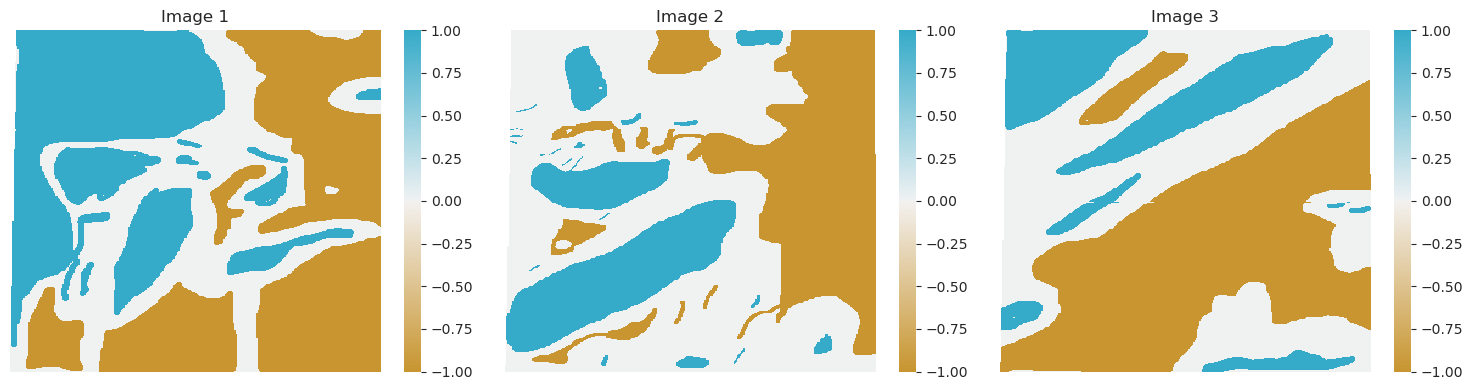
\includegraphics[width=1.0\textwidth]{1.a.png}
\caption{Three data units taken at different times at the same Arctic location. Each pixel is color-coded by its respective expert label. Cloudy for \textcolor{BlueGreen}{blue}, \textcolor{Tan}{Brown} for surface, and White for unlabeled pixels.}
\label{fig:image_labels}
\end{figure*}

We first plot the spatial distribution of labels image-wise. This is shown in Figure \ref{fig:image_labels}, where we have plotted each of the three images overlaid with their associated class. As can be seen, especially in image 2 and image 3, many pixels are unlabelled. Further, the placement of labeled pixels also varies according to the images. This is further captured in Figure \ref{fig:label_dist}, which shows that the proportionality between the three classes varies significantly across images. Image 2 has a majority of points unlabelled, but image 1 has the majority of points labeled. Given the variations among the Satellite images, a reasonable classifier should be able to handle unbalanced classes while simultaneously generalizing well to a whole range of unseen Arctic satellite images --- one with absolutely no cloud or full cloud coverage.

\begin{figure}[!h]
\centering
% \captionsetup{justification=centering}
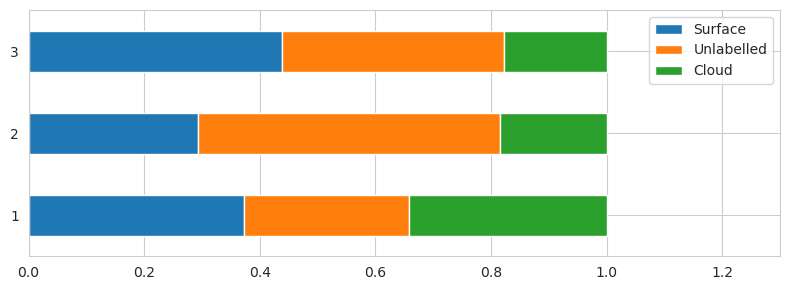
\includegraphics[width=0.48\textwidth]{2.a.png}
\caption{Label distribution percentages for the three images in our dataset}
\label{fig:label_dist}
\end{figure}

The dispersion of labels also shows how highly correlated the labels are to the spatial location of the images. We can see large patches of pixels in all three images with the same label. This tells us that nearby pixels in the same image are likely to have the same labels. For example, if we predict by using the neighboring pixel, we can do extremely well due to data leakage. Hence, if we blindly do the model training using the typical randomized K-folds, the resulting scores are not that informative. In other words, the usual i.i.d samples assumption is inappropriate here; we must be particularly cautious about this in the training procedure.


\subsection{Covariate Signals}
We first investigate the distribution between the 3 expert engineered features, NDAI, CORR, and SD\footnote{SD has a much larger range than the rest; thus, we applied a log transformation for plotting purposes.}. Figure \ref{fig:covariate_pairplot} provides a pair plot of the 8 covariates, in either 1-D or 2-D KDE plots, that are available to us. We can see that all engineered features provide some signals from a different angle, and all the raw radiance measurements add little to no signal to the classification problem.

We notice a few interesting facts starting at the diagonal 1-D KDE plots. Most surface pixels have NDAI less than 0, CORR less than 0.25, and lower SD. NDAI alone provides an outstanding separability out-of-box. By plotting NDAI against SD, we see the two classes are already on their own distinct density mass with a slight overlap. The subplot in column 3 and row 1, CORR, adds more information by stating that Cloud particles tend to have a higher spatial correlation. The surface particles have a low correlation across the spectrum, less than $0.25$. And the cloud particles, on the other hand, tend to have a higher correlation greater than $0.25$.

Next, we plot the features spatially with each pixel in its x-y coordinate overlaid with the three most influential features, NDAI, Corr, and Log(SD), in Figure \ref{fig:spatial_dist_covariates}. Firstly, we see that the values of the features are highly spatially correlated, meaning that neighboring pixels tend to have similar values. This is unsurprising since the expert features are derived based on a convolution kernel of either a 5x5 or 8x8 around the neighboring pixels. Interestingly we also observed that there is not one expert-engineered feature that perfectly aligns with all the labeled values in all the 3 images. That is to say that a high-performing classifier will likely need to use a combination of the features because a linear separating hyperplane does not exist.

\begin{figure*}[!h]
\centering
% \captionsetup{justification=centering}
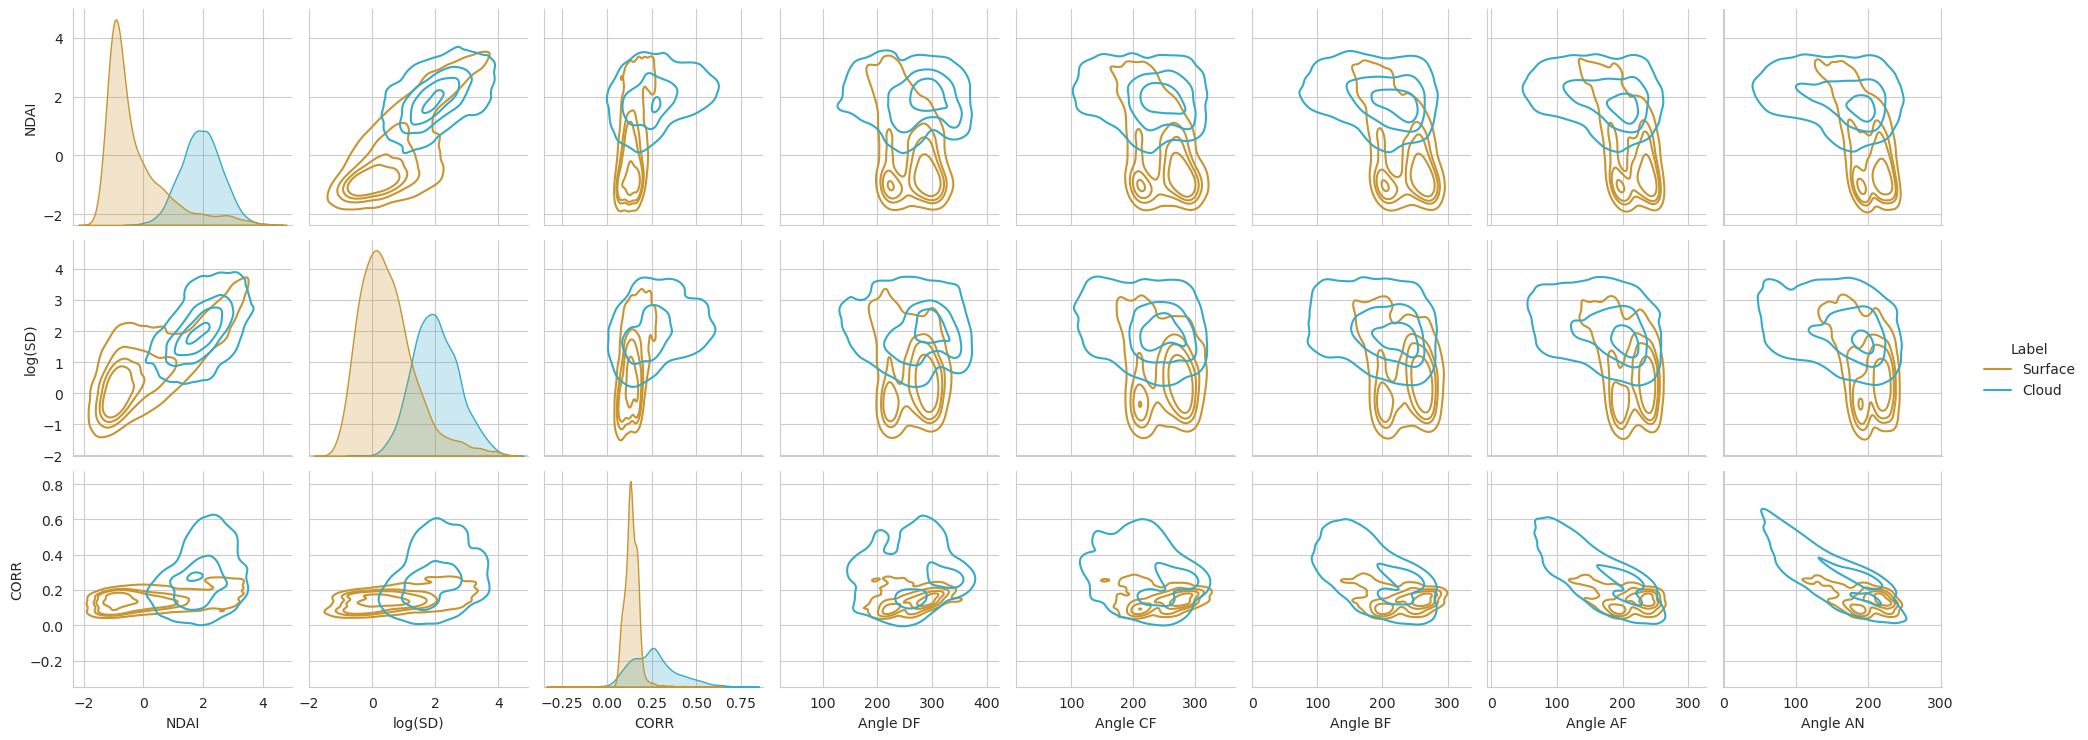
\includegraphics[width=1.04\textwidth]{2.c.png}
\caption{Pair plot of all 8 features}
\label{fig:covariate_pairplot}
\end{figure*}

\begin{figure}[!h]
\centering
% \captionsetup{justification=centering}
\includegraphics[width=0.5\textwidth]{image_spatial_features.png}
\caption{Each image overlaid with values for NDAI, CORR, and Log(SD). Red represents high values and blue low values}
\label{fig:spatial_dist_covariates}
\end{figure}


\section{Preparation}

\subsection{Data Splitting}
Most out-of-box cross-validation (CV) methodology assumes i.i.d samples, which do not play well with the images that inherently contain spatial-temporal correlation. For instance, images can be taken at the same location but at different times, and neighboring pixels are highly correlated with each other. Image pixels are not i.i.d samples. If we are not careful with our training procedure, we can introduce unwarranted data leakage and unjustified scores. To alleviate the potential data leakage issue, we propose two specialized cross-validate-test (CVT) strategies to handle this spatial dependence shown in Figure \ref{fig:test_schema}.

\begin{figure*}
    \centering
    \subfloat[\centering Test Schema 1]{{ 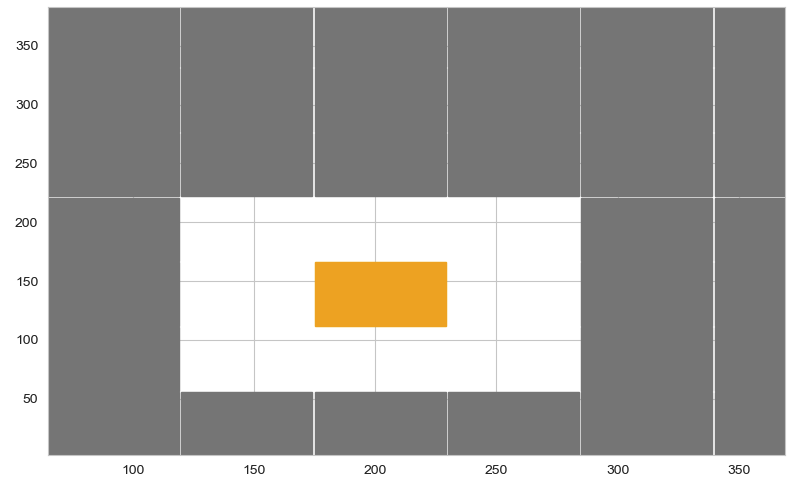
\includegraphics[width=0.5\textwidth]{test_scheme1.png} }}
    \subfloat[\centering Test Schema 2]{{ 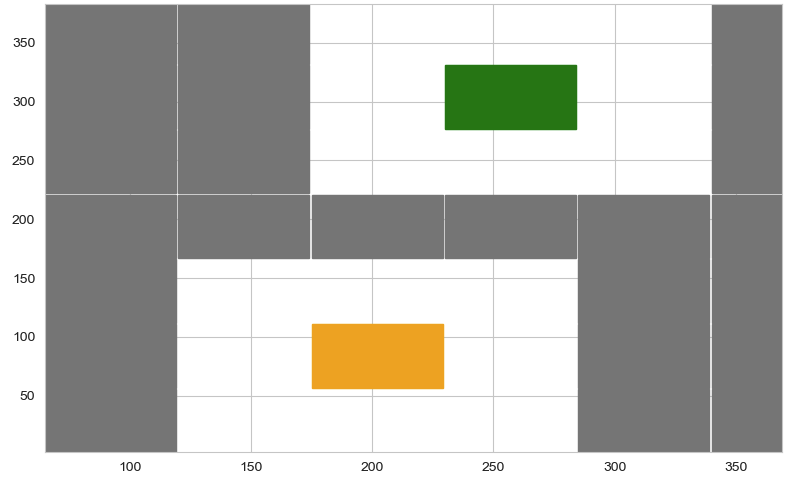
\includegraphics[width=0.5\textwidth]{test_scheme2.png} }}
    \caption{Two different CVT methods. \textcolor{Gray}{Gray} patches represent training data, \textcolor{orange}{orange} patches represent validation data, and \textcolor{ForestGreen}{green} patches represent test data.}%
    \label{fig:test_schema}%
\end{figure*}

\subsubsection{CVT Scheme 1}
With only 3 image units given, we first keep image 1, the one with most of the pixels labeled, out for our testing set, then use the other 2 images for the training and validation set. The procedure is illustrated in the left plot of Figure \ref{fig:test_schema}. In other words, we train and tune our models using only 2 images and test on the last image. Then, we pick a $55\times55$ kernel size that defines our validation set, shown in \textcolor{orange}{orange}, and remove the surrounding pixels of the kernel completely from the training set, shown in the white spaces. If used in training, the white region represents omitted data points, as these points will contain information about the pixels in the validation/test set. Then, the remaining gray area is the training set. Note this CV procedure is applied on the 2 training images simultaneously and at the same patch. It is important because taking validation patches at different areas can potentially introduce leakage if the two images were shot at the same location. Lastly, the validation patch shifts around the image, with each shift forming a cross-validation (CV) fold. Although it is not the best use of limited data, it ensures there is no data leakage through spatial dependencies. 

\subsubsection{CVT Scheme 2}
The validation approach remains the same in these strategies, but the testing method differs in the second Scheme. We introduce a nested approach to make the most use of the limited data. In other words, we can train, validate, and test each at the same time each fold instead of keeping one testing image out completely. To illustrate, the right plot of Figure \ref{fig:test_schema} contains an example. With this procedure, we can use all 3 images as a combined training, CV, and test set. Here we have an additional \textcolor{ForestGreen}{green} patch representing our test set only with the \textcolor{orange}{orange} validation set. We segment a part of the image at each fold and use it in testing. While both patches shift around the image, everything else stays the same, 

\subsection{Baseline}
We compute the accuracy of a trivial classifier for both test schemes, which sets all labels to cloud-free. These results are reported in Table \ref{tab:scheme1_results}. We see that a naive classifier that predicts all pixels are surface achieves around 52\% accuracy, which is well underperforming from the rest of the classifiers. Such exercise sets the baseline that our result is not trivial.

\subsection{First Order Importance}
In section 2.B, we covered the importance of features, which is also shown in Figure \ref{fig:covariate_pairplot}. Here we are just reciting the content to highlight that the 3 expert-engineered features are well-designed. We can achieve pretty far on the classification task by only using the expert-engineered features, NDAI, CORR, and SD. We can see in the KDE plot of NDAI and SD that surface and cloud pixels form distinct density mass with a slight overlap. Adding CORR into the mix by identifying pixels with low correlation are typically surface pixels, we can achieve a reasonable result that should resemble a logistic regression using only these 3 features.


\section{Modeling}
\subsection{Models Considered}
% Results 1 table
\begin{table}
\begin{center}
\resizebox{\columnwidth}{!}{
\begin{tabular}{||c | c c c c||} 
    \hline
    Model & CV Acc. & CV B.Acc. & Test Acc. & Test B.Acc. \\ [0.5ex] 
    \hline\hline
    Baseline & 0.616 & 0.523 & 0.522 & 0.522 \\ 
    \hline
    LR & 0.880 & 0.869 & 0.929 & 0.929 \\ 
    \hline
    RF& 0.879 & 0.879 & 0.911 & 0.912 \\
    \hline
    CART & 0.872 & 0.868 & 0.856 & 0.858 \\
    \hline
    Adaboost & 0.884 & 0.874 & 0.934 & 0.938 \\
    \hline
\end{tabular}
}
\caption{CV and test results for the 4 models under test scheme 1. "B.Acc" stands for balanced accuracy.}
\label{tab:scheme1_results}
\end{center}
\end{table}

% Results 2 Table
\begin{table}
\begin{center}
\resizebox{\columnwidth}{!}{
\begin{tabular}{||c | c c c c||} 
    \hline
    Model & CV Acc. & CV B.Acc. & Test Acc. & Test B.Acc. \\ [0.5ex] 
    \hline\hline
    Baseline & 0.603 & 0.537 & 0.603 & 0.537 \\ 
    \hline
    LR & 0.877 & 0.820 & 0.877 & 0.820 \\ 
    \hline
    RF& 0.879 & 0.846 & 0.878 & 0.845 \\
    \hline
    CART & 0.860 & 0.822 & 0.860 & 0.822 \\
    \hline
    Adaboost & 0.867 & 0.805 & 0.867 & 0.805 \\
\hline
\end{tabular}
}
\caption{CV and test set results for the 4 models under test scheme 2}
\label{tab:scheme2_results}
\end{center}
\end{table}

For the next couple of sections, we compare 4 different classification methods, logistic regression (L2 regularized), CART, Random Forest, and Adaboost, on the cloud detection task. We provide some brief commentary on the assumptions of these well-known models. Besides, all these models assume i.i.d samples. We know that they are not due to spatial dependence. However, as mentioned previously, we have addressed the spatial correlation issue with our specially designed CVT procedures. 
\begin{itemize}
    \item \underline{Logistic Regression}. This model assumes a linear decision boundary between the two classes. According to our EDA, we should expect it to achieve a reasonable result since the data seems well separated linearly using just the 3 expert-engineered features. However, we cannot be sure about the high-dimensional space.
    \item \underline{CART}. This model is non-linear and partitions the feature space into rectangles. In particular, it will perform worse if the decision boundary is not axis aligned. 
    \item \underline{Random Forest}. This model is non-linear and uses bootstrap aggregation to reduce variance. Another important point is that the model works better when the set of trees trained is less correlated. One factor that affects this is if different covariates used are correlated. This is something that affects us since we use all 8 features, but we know that 3 of the features (NDAI, CORR, and SD) actually are transformations of the other 4.
    \item \underline{Adaboost}. This model is also non-linear and uses boosting to overcome the limitations of a single weak classifier. In this case, we use a pruned CART tree, with only 1 depth, as the weak learner. Not many assumptions of this model affect our use of it.
\end{itemize}


\subsection{CV Results}
\label{sec:cv_results}
We use patch sizes of 55x55. In total, this produces 44 folds for cross-validation for test scheme 1. And 40 folds for cross-validation/testing in test scheme 2. We consider two metrics, accuracy and balanced accuracy, for computing the CV errors and test errors for both test schemes. Aggregated validation and test results are provided in Tables \ref{tab:scheme1_results} and \ref{tab:scheme2_results} for test schemes 1 and 2, respectively. In general, all the machine learning models perform well, far exceeding the simple baseline model. For test scheme 1, we can see that Adaboost performs the best in both cross-validation and in test set accuracy and balanced accuracy. This, however, is not the same in test scheme 2, where Random forest performs the best in both cross-validation and in test set accuracy and balanced accuracy. Interestingly, we can also see that the simple logistic regression model, the only linear model out of the candidate models, performs well in both test schemes, being the second-best-performing model in test scheme 1 and test scheme 2. This is likely due to the presence of expert-engineered features, which Tao's team has shown to be highly predictive of cloud presence through their ELCM algorithm.

These tables also show the difference between test scheme 1 and test scheme 2. We can see that the CV results and the test results are very similar in test scheme 2 (as seen from Table \ref{tab:scheme2_results}), whereas the test results in Table \ref{tab:scheme1_results} are generally worse than the CV results. This reflects the fact that test scheme 2 eventually uses the same data set; hence, we expect both to produce similar scores. In contrast with test scheme 1, the test procedure (testing on 1 image) is quite different from the validation procedure. We see that test scheme 1 allows us to detect the overfitting of some models even when high CV accuracy is shown. This is the case in the Random Forest model, which had the second-best performing CV accuracy, but the poorest test accuracy.

More insights can be gleaned from Figures \ref{fig:fold_results_1} and \ref{fig:fold_results_2}, which plot the individual fold errors. Things to note here are that the errors fluctuate a fair bit over the different folds. This is due to our patch-wise formation of the validation set, meaning that the labels in most patches will be similar. In subsequent sections, we systematically analyze whether our model makes errors on certain labels. 

\begin{figure}[h]
\centering
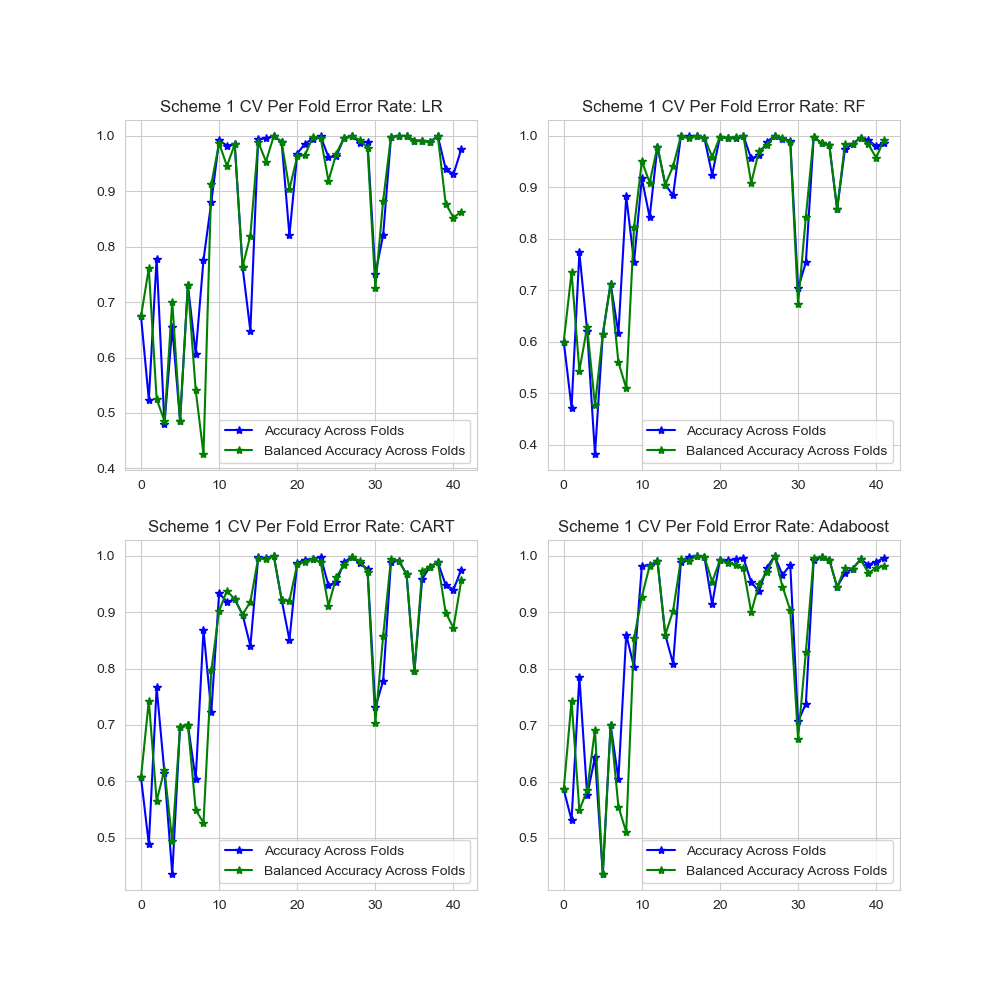
\includegraphics[width=0.5\textwidth]{statics/test_Scheme_1_Fold_error.png}
\caption{Accuracy and Balanced Accuracy for each validation fold in Test Scheme 1. Top left: Logistic Regression, Top Right: Random Foret, Bottom Left: CART, Bottom Right: Adaboost}
\label{fig:fold_results_1}
\end{figure}

\begin{figure}[h]
\centering
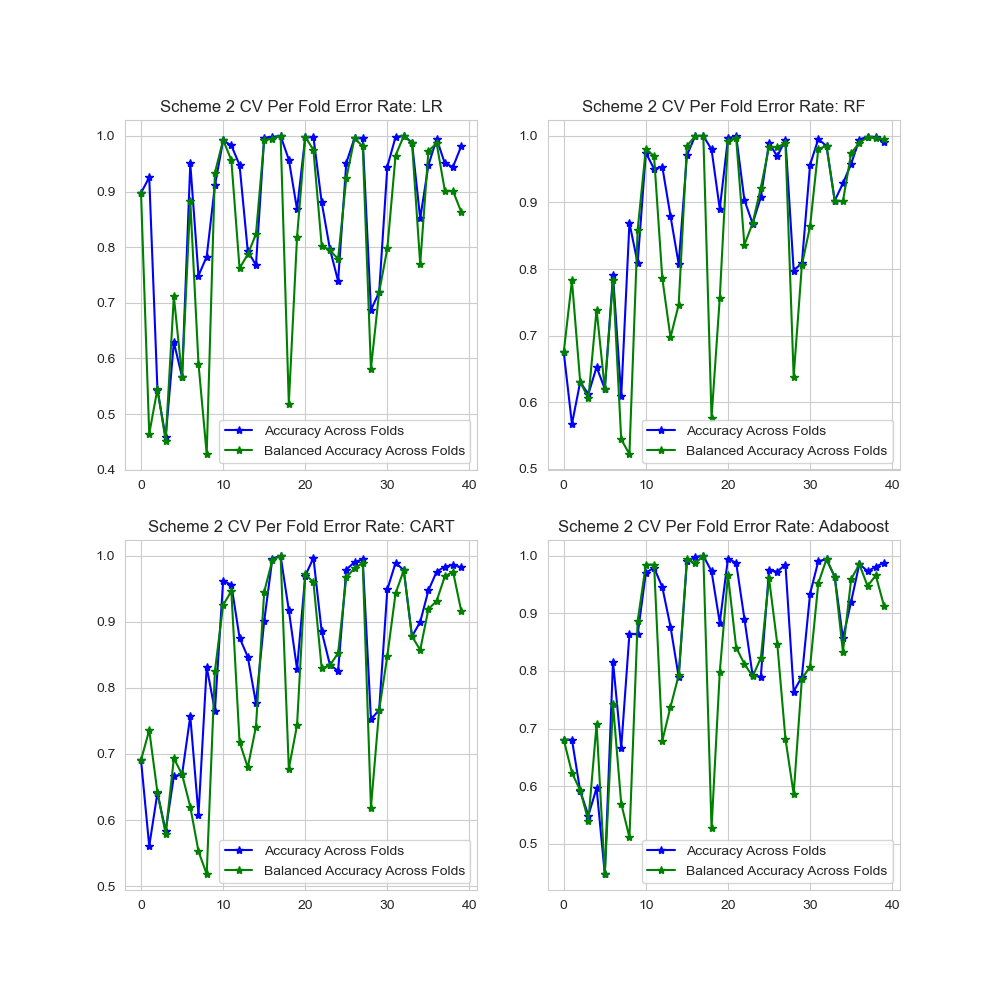
\includegraphics[width=0.5\textwidth]{statics/test_Scheme2_fold_error.png}
\caption{Accuracy and Balanced Accuracy for each validation fold in Test Scheme 2. Top left: Logistic Regression, Top Right: Random Foret, Bottom Left: CART, Bottom Right: Adaboost}
\label{fig:fold_results_2}
\end{figure}


\subsection{ROC Plots}
\begin{figure}
    \centering
    \subfloat[\centering Test Scheme 1: CV ROC]{{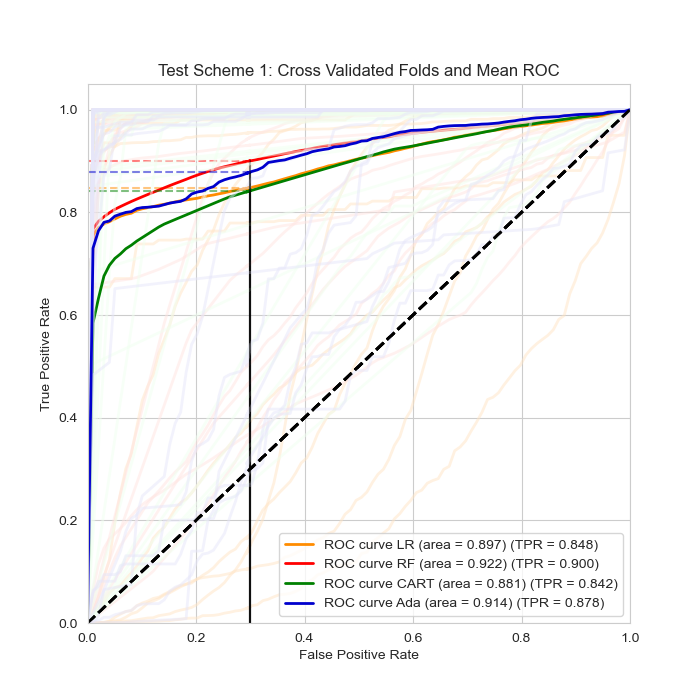
\includegraphics[width=0.375\textwidth]{statics/test_Scheme1_cv_roc.png} }}
    \qquad
    \subfloat[\centering Test Schema 1: Test ROC]{{
\includegraphics[width=0.375\textwidth]{statics/test_Scheme1_test_roc.png} }}
    \caption{Left: ROC curves per fold and Mean ROC curve for the 4 models. Right: ROC curves of the single held-out test set for the 4 models.}
    \label{fig:ROC_curves scheme1}
\end{figure}

\begin{figure}
    \centering
    \subfloat[\centering Test Scheme 2: CV ROC]{{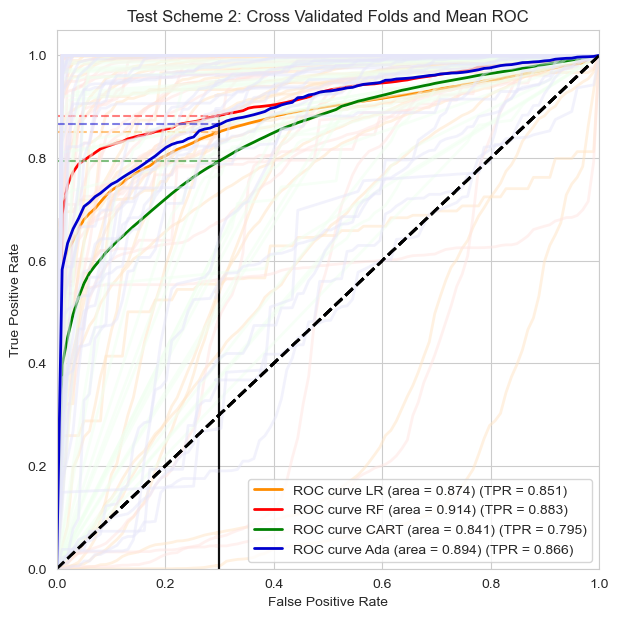
\includegraphics[width=0.375\textwidth]{statics/test_Scheme2_cv_roc.png} }}
    \qquad
    \subfloat[\centering Test Schema 2: Nested Test ROC]{{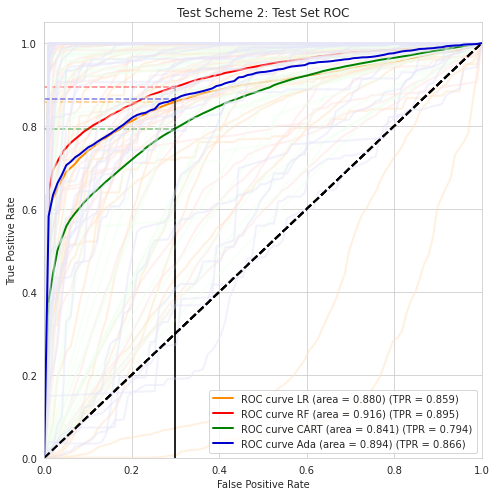
\includegraphics[width=0.375\textwidth]{statics/test_Scheme2_test_roc.png} }}
    \caption{Left: ROC curves per fold and Mean ROC curve for the 4 models. Right: ROC curves of each test fold and Mean ROC curves across all test folds for the 4 models.}
    \label{fig:ROC_curves scheme2}
\end{figure}

We plot the ROC curves generated for both the validation and test set(s) used in testing scheme 1 and testing scheme 2. These are displayed in Figure \ref{fig:ROC_curves scheme1} and \ref{fig:ROC_curves scheme2}. For cross-validation ROC and test scheme 2 ROC, we plot the mean ROC curves over ROC curves generated by each fold. A ROC curve highlights the predicted true positive rate a model can achieve for a given false positive rate (or vice versa). With the cloud class as the "true" class, a high true positive rate implies that a pixel that is actually a cloud will high a high chance of being classified as a cloud. This conflicts with the objective of a low false positive rate which measures how often non-cloud pixels are predicted as clouds. Intuitively, a model with a more favorable trade-off between the two is better performing; this can be measured by the area under the curve metric (AUC).

Under test scheme 1, we see a noticeable difference in AUC between cross-validation and testing, with the test set AUCs being higher for all models except CART. We see that under test scheme 1, Adaboost has the most favorable test AUC, which again matches the observations in section \ref{sec:cv_results}.

For test scheme 2, the AUC from all 4 models between CV and test is very similar. This is due to the same reasons highlighted earlier about the similarity between the CV and testing in test scheme 2. Under test scheme 2, Random forest has the most favorable trade-off, with the best AUC. LR and Adaboost perform similarly, and CART has a noticeably lowered AUC compared to the other 3 models, which is not surprising. These results parallel what was observed in the metric-based evaluation in section \ref{sec:cv_results}.

Next, we fix the False Positive Rate (FPR) and compute the True Positive Rate (TPR) based on the induced threshold needed to obtain that FPR rate. This allows an end user to fix an acceptable level of false positive rate. We demonstrate an example of a low false positive rate, set at 0.3. We see that for this, most models can attain a TPR above 0.8 under both test schemes. Such a choice of a lower FPR would reflect for the case where it is more important to correctly capture the presence of all the cloud pixels, which might be the case if the model was applied some weather monitoring purpose.


\section{Diagnostics}
We base our choice of the model on performance on testing scheme 1. This is because testing scheme 1 better reflects the actual use case of the model, where inference will be made on a set of whole new images. Hence we choose the Adaboost model, which has the best validation and test performance in test scheme 1.

\subsection{Analysis of Adaboost}
\begin{figure}[h]
    \centering
    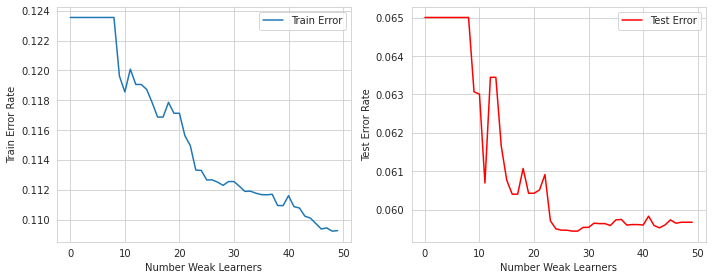
\includegraphics[width=0.5\textwidth]{statics/ada_iterations_tr_23_te_1.png}
    \caption{Percentage error across subsequent iterations of Adaboost. Left: Error on Train Set, Right: Error on Test Set.}
    \label{fig:Adaboost_iterations}
\end{figure}

\begin{figure}[h]
    \centering
    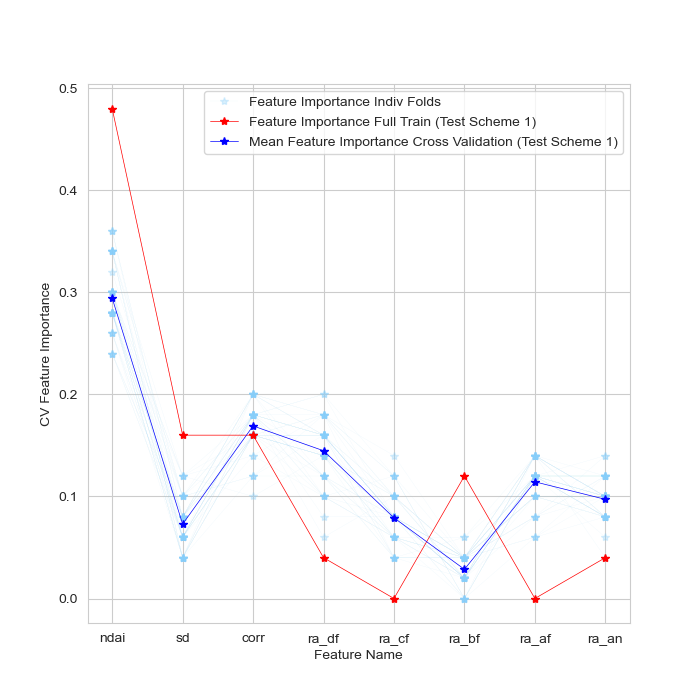
\includegraphics[width=0.5\textwidth]{statics/Feature_importance_test_scheme1_tr_23_te_1.png}
    \caption{Feature Importance of Adaboost for 1) model trained on full train and validation set. 2) Each CV fold 3) Average across CV folds.}
    \label{fig:Feature_importance ts1}
\end{figure}

We look at the sequence of error rates generated by the boosting algorithm to analyze the convergence. We also analyze the feature importance to check for stability in the chosen features over the various validation folds and train sets.

\subsubsection{Convergence Analysis}
Being an iterative algorithm, we first assess the performance of the AdaBoost learner across each iteration. This is displayed in Figure \ref{fig:Adaboost_iterations}. We see that the algorithm's test error converges, decreasing rapidly and then rising after just 25 boosting iterations. More boosting iterations are likely to result in overfitting of the training set. We believe that the algorithm converges with so few boosting iterations because the expert-engineered features provide a large amount of information to the model. As can be seen, even the initial decision stump can achieve close to 12.4\% train error.

\subsubsection{Feature Importance}
Next, we assess the stability of the Adaboost model via its learned feature importance. This feature importance score is calculated by aggregating, for a trained Adaboost model, the feature importance of each weak learner (decision tree) learned by the algorithm. We calculate feature importance in test scheme 1 for 1) the Model trained on the full train/validation set and 2) the Model trained at each cross-validation fold. These results are shown in Figure \ref{fig:Feature_importance ts1}. Comparing the learned feature importance, we see that the model learned on the full training set generally matches those learned in the cross-validation models. For example, NDAI is consistently the highest-ranked feature. Likewise, CORR is ranked highly in both the testing and cross-validation models. This similarity in feature importance indicates model stability across the various data splits and with the final test model. 

\subsection{Analysing Error Patterns}
\begin{figure}
    \centering
    \subfloat[\centering Test - Image 1]{{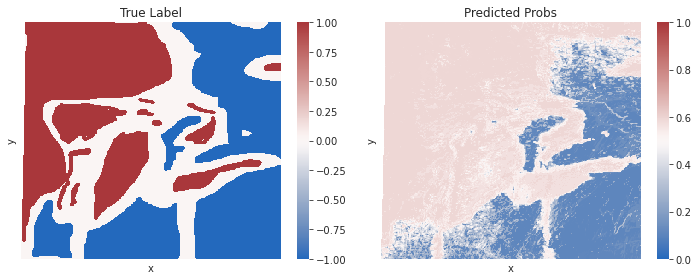
\includegraphics[width=0.425\textwidth]{ada_test_prob_tr_23_te_1.png} }}
    \qquad
    \subfloat[\centering Train - Image 2]{{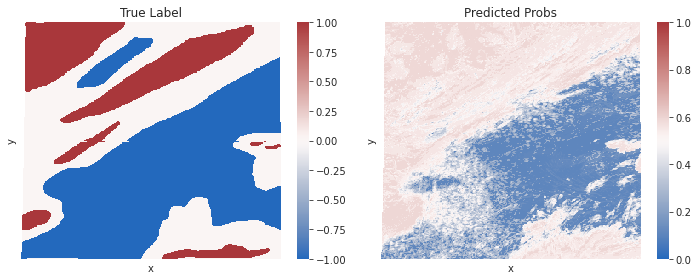
\includegraphics[width=0.425\textwidth]{ada_train_prob1_tr_23_te_1.png} }}
    \qquad
    \subfloat[\centering Train - Image 3]{{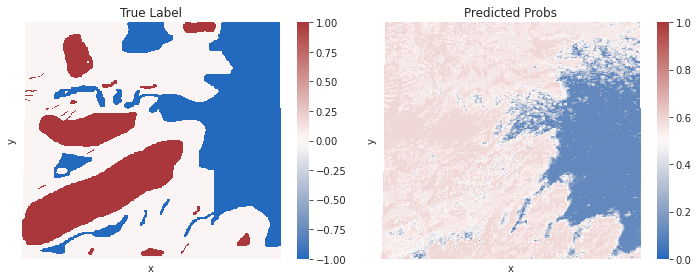
\includegraphics[width=0.425\textwidth]{ada_train_prob2_tr_23_te_1.png} }}
    \caption{Left Column: Pixels colored by expert labels, Red: Clouds, Blue: No Clouds, White: Unlabelled. Right Column: Predicted probability given by the model.}
    \label{fig:Probability_Preds}
\end{figure}

\begin{figure*}[!h]
    \centering
    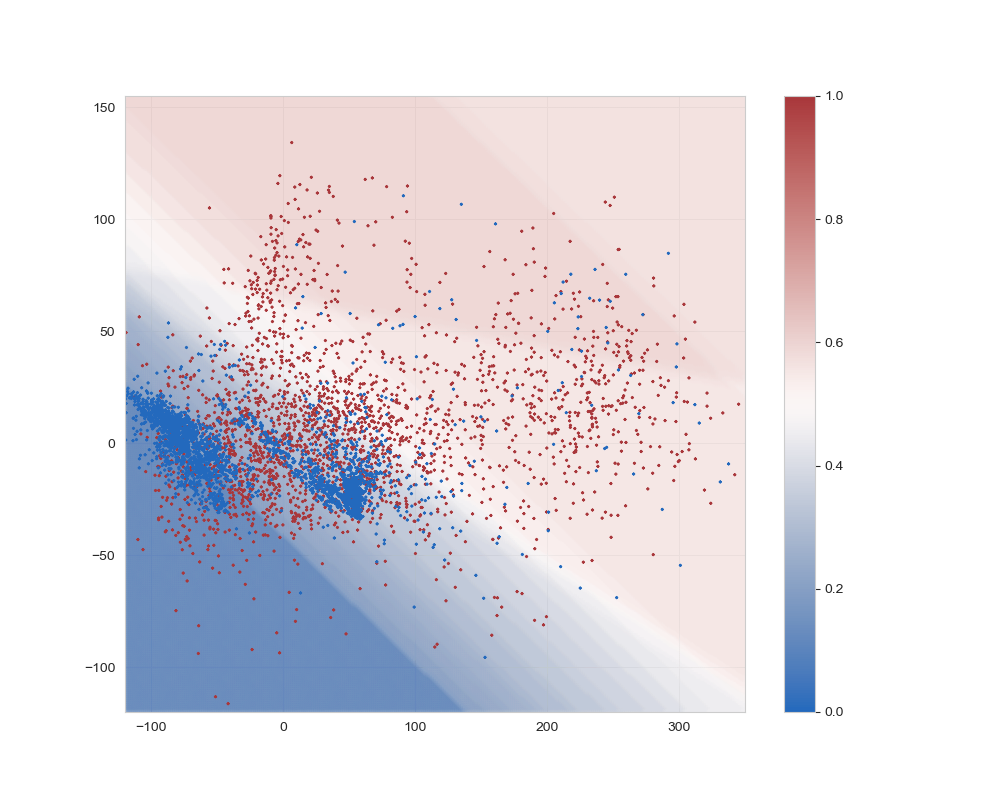
\includegraphics[width=0.4\textwidth]{statics/PCA_decision_surface_tr_23_te_1.png}
    \qquad
    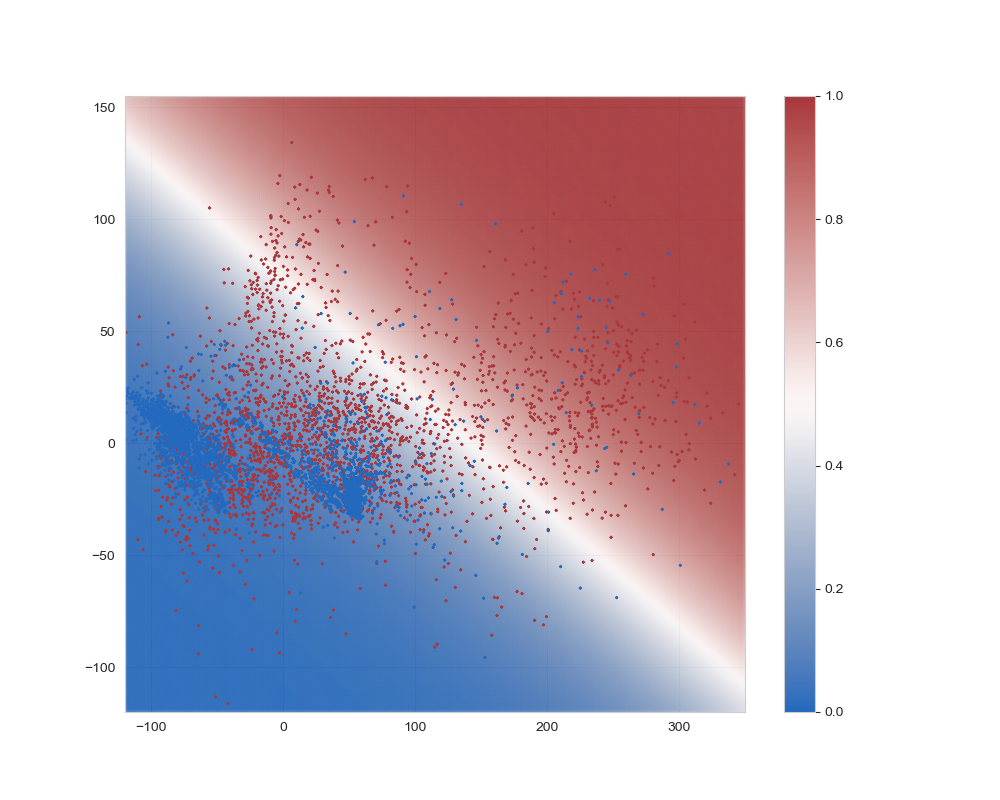
\includegraphics[width=0.4\textwidth]{statics/log_reg_decision_surface_tr_23_te_1.png}
    \caption{Decision Surfaces of Adaboost (Left) and Logistic Regression (Right). The decision surfaces were conducted under a low-dimension feature space projection using PCA.}
    \label{fig:decision_surface}
\end{figure*}

We analyze error patterns mainly by looking at the predicted probabilities across different spatial regions and regions in the feature space. The latter poses challenges due to the high dimensional nature of the feature space. We describe in subsequent sections how we overcame this using dimensionality reduction methods.

\subsubsection{Prediction Probabilities}
We first investigate how well-calibrated the predicted probabilities generated by Adaboost are. This gives us insights into how the algorithm performs. For each image, we generate predictions of the probability of a cloud prediction for each pixel. We then compare this to the true expert-labeled pixels. These are plotted in Figure \ref{fig:Probability_Preds}. Firstly for the training case, we can see clearly that across images 2 and 3, there are more non-cloud labeled points than cloud points. This creates a bias in the training data. Interestingly we see that the model seems biased toward predicting a pixel as a cloud, with large swaths of the image's predicted probability slightly greater than 0.5. For example, in the first training image, misclassification occurs in non-cloud regions being predicted as clouds in areas where the non-cloud regions are surrounded by clouds, where the transition occurs. The same is seen in the second training image, where only the rightmost patch of non-cloud regions is successfully predicted by the AdaBoost algorithm. Another point to note is that the model is generally very cautious about its probability prediction for the cloud class, with the highest predicted probability being only 0.61. In contrast, it is more confident about predicting a non-cloud, with predictive probabilities reaching 0.113. This is reflected in Figure \ref{fig:Probability_Preds}, where the red probability regions are very faint, and the blue probability regions are darker. This is a positive feature of the model since the train set generally has fewer cloud-labeled points; hence it is natural that the model should generally be less confident about predicting points as the cloud class. In contrast, since the dataset has relatively more non-cloud classes, the model has become more confident when predicting them. In other words, the model found predicting the surface pixels much easier. Thus we have reason to believe that given more training data, the model will become more confident about its cloud class prediction.

\begin{figure}[!h]
    \centering
    \subfloat[\centering Histograms of NDAI (Left), Corr (Center), and SD (Right), between misclassified and correctly classified \textbf{Surface} (Non-Cloud) data points. \textcolor{blue}{Blue} histograms represent the distribution of features of points that are correctly classified and \textcolor{orange}{orange} those that are mis-classified]{{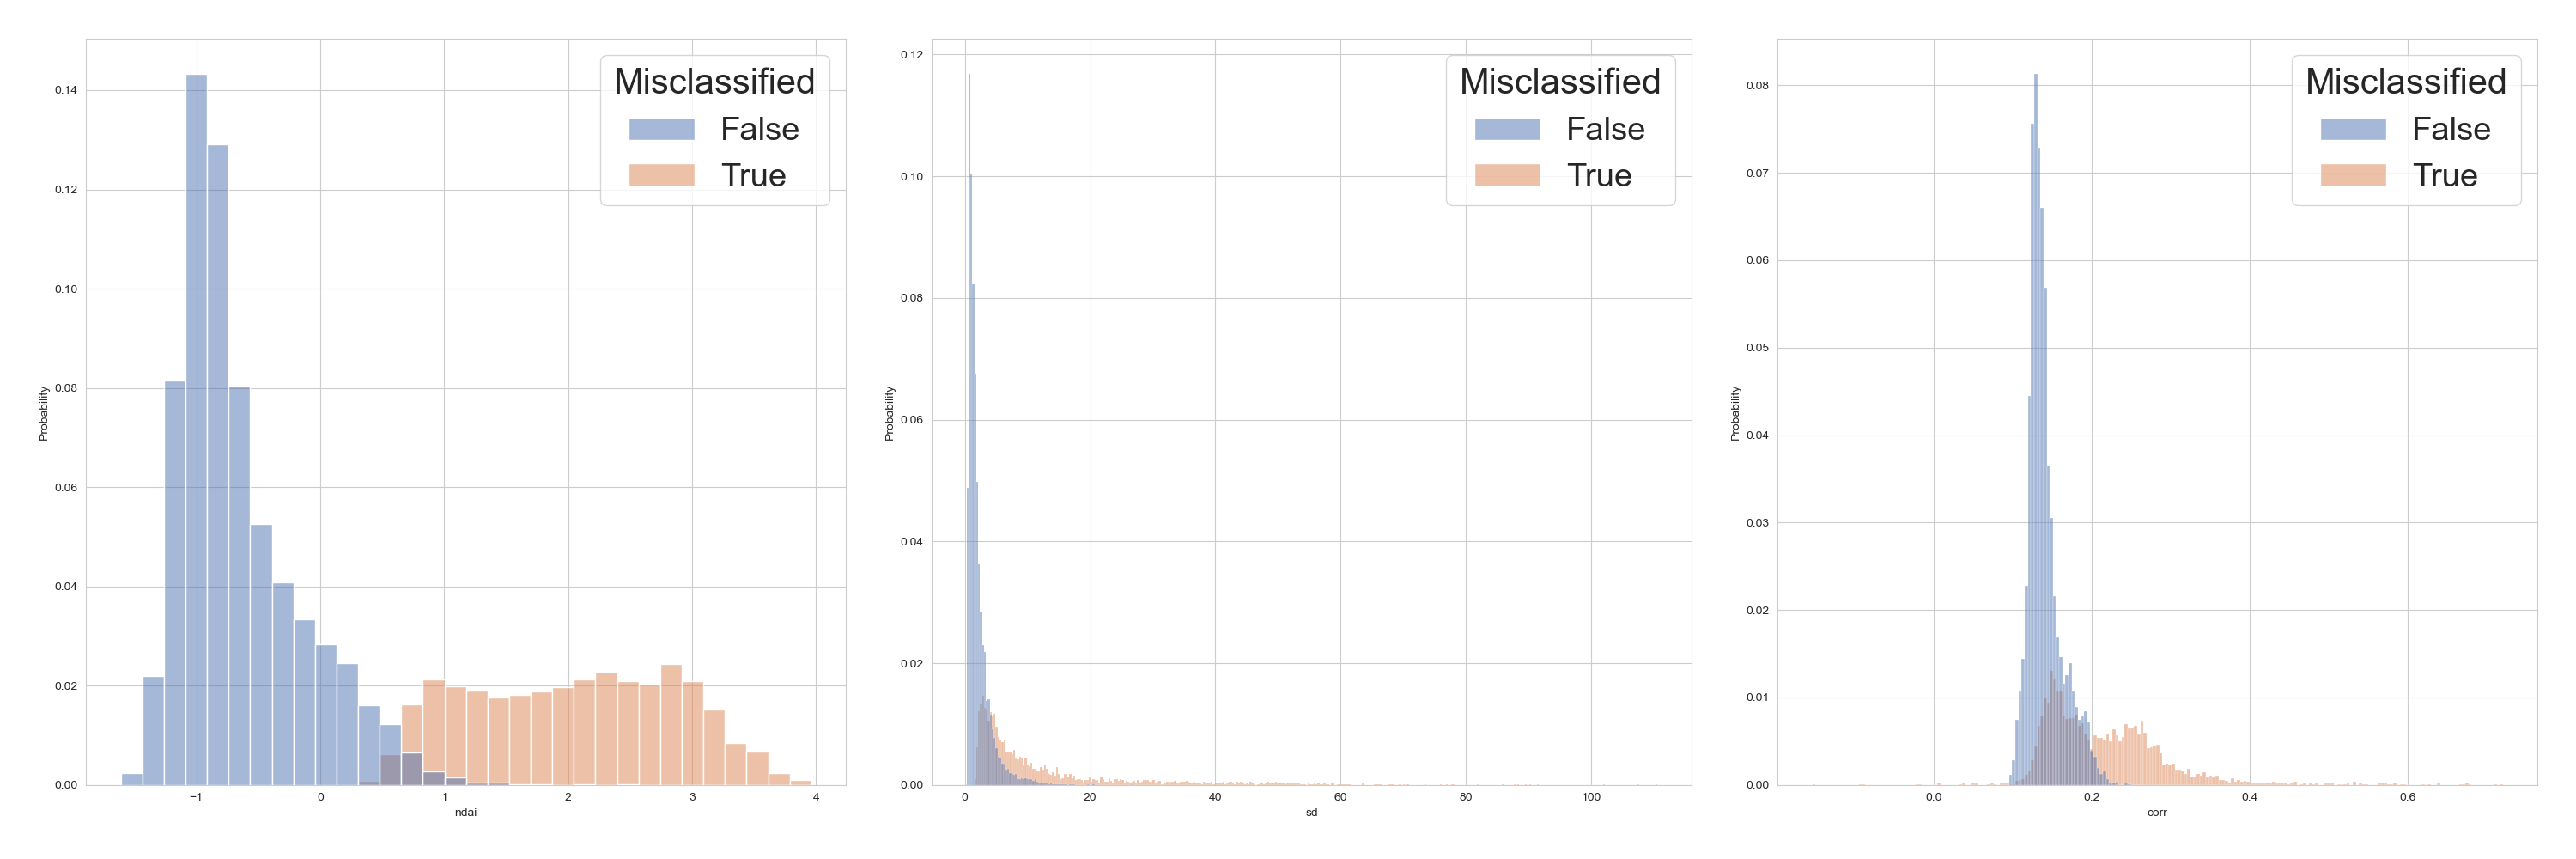
\includegraphics[width=0.5\textwidth]{statics/feature_compare_true_neg_tr_23_te_1.png} }}
    \qquad
    \subfloat[\centering  Histograms of NDAI (Left), Corr (Center), and SD (Right), between misclassified and correctly classified \textbf{Cloud} data points. \textcolor{blue}{Blue} histograms represent the distribution of features of points that are correctly classified and \textcolor{orange}{orange} those that are mis-classified]{{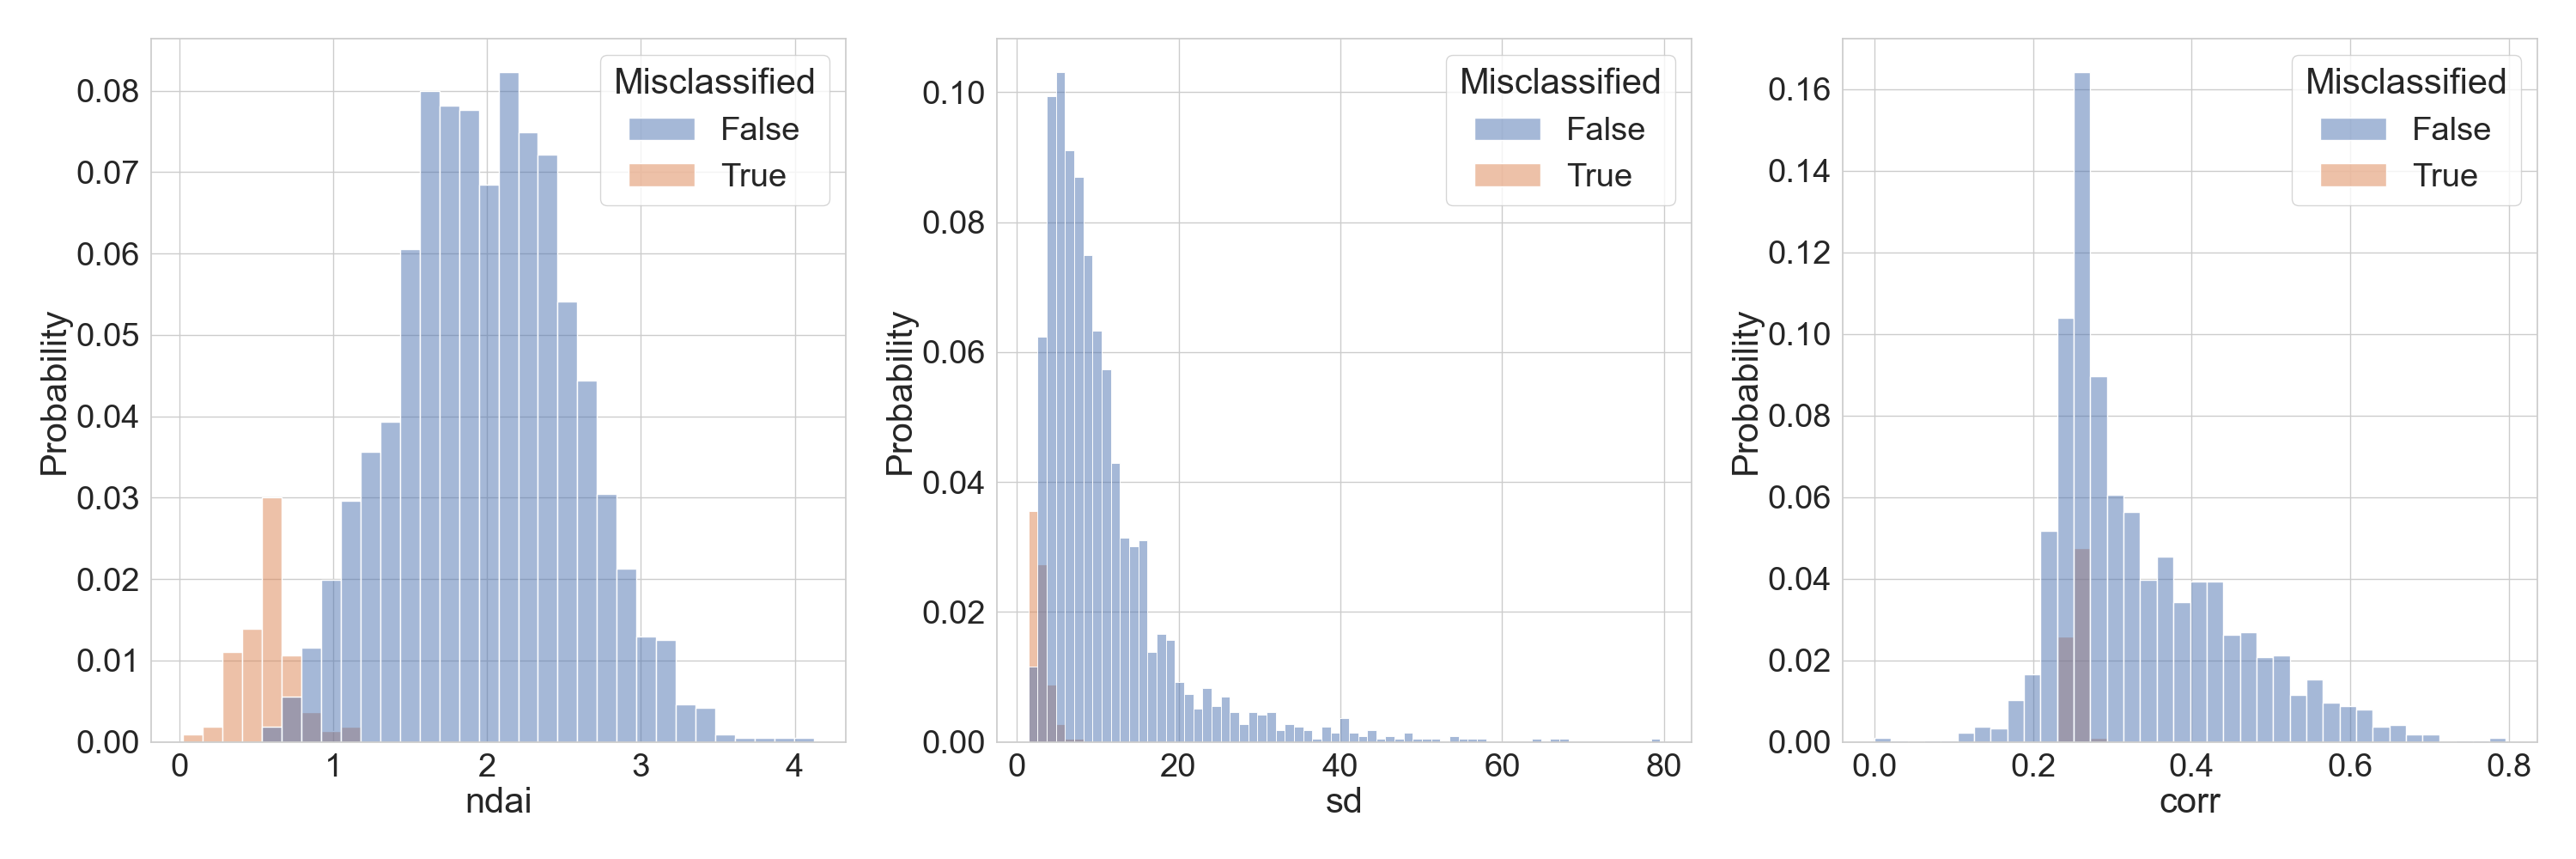
\includegraphics[width=0.5\textwidth]{feature_compare_true_pos_tr_23_te_1.png} }}
    \caption{Feature Value Histograms for NDAI, Corr, and SD overlaid with colors indicating whether the model correctly or incorrectly classified them. Top: Histograms for cloud-labeled pixels. Bot: Histograms for surface (non-cloud) labeled pixels}
    \label{fig:feature_val_compare}
\end{figure}

\begin{figure*}[!h]
    \centering
    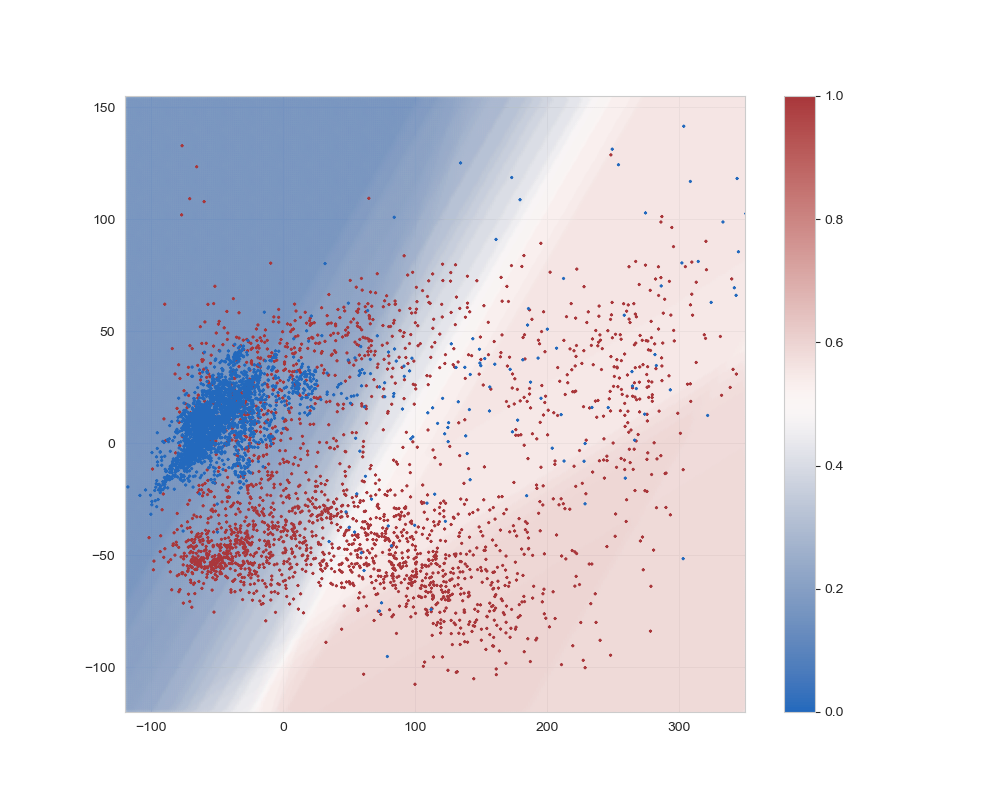
\includegraphics[width=0.4\textwidth]{statics/PCA_decision_surface_tr_12_te_3.png}
    \qquad
    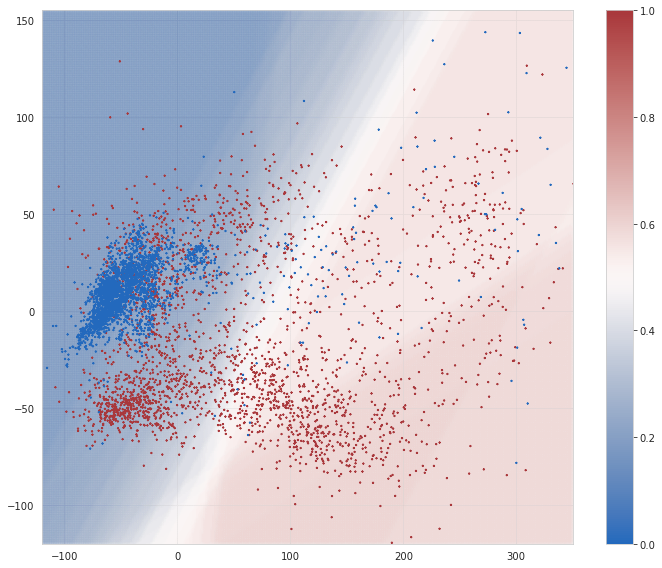
\includegraphics[width=0.4\textwidth]{statics/log_reg_decision_surface_tr_12_te_3.png}
    \caption{Decision Surfaces of Adaboost (Left) and Logistic Regression (Right). The decision surfaces were conducted under a low-dimension feature space projection using PCA.}
    \label{fig:decision_surface_alt}
\end{figure*}

\begin{figure}
    \centering
    \subfloat[\centering Test - Image 3]{{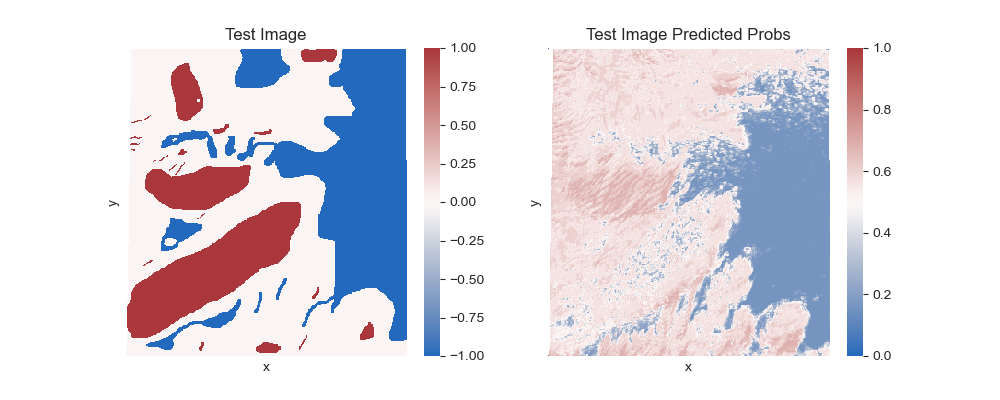
\includegraphics[width=0.425\textwidth]{ada_test_prob_tr_12_te_3.png} }}
    \qquad
    \subfloat[\centering Train - Image 1]{{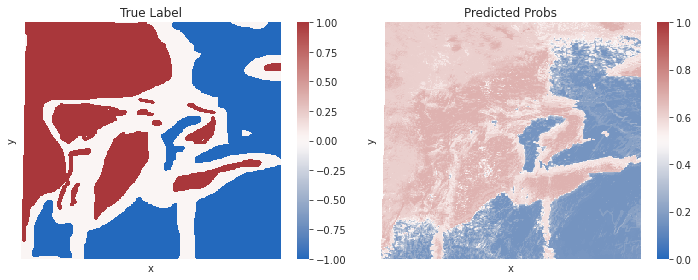
\includegraphics[width=0.425\textwidth]{ada_train_prob1_tr_12_te_3.png} }}
    \qquad
    \subfloat[\centering Train - Image 2]{{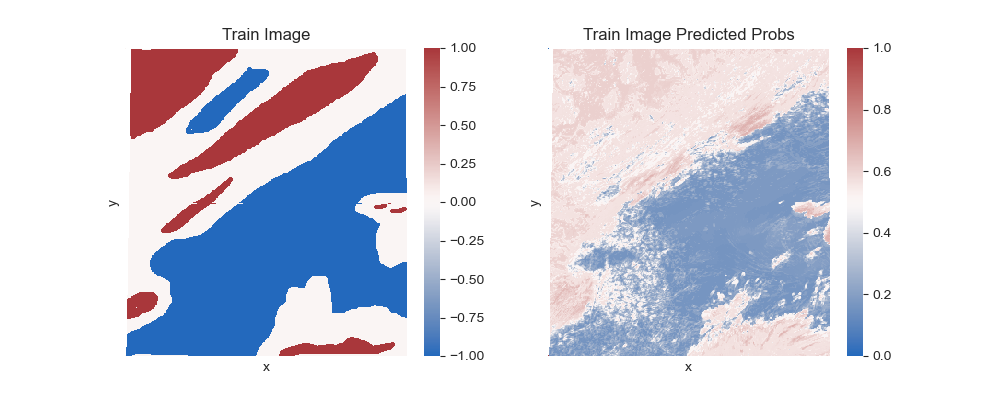
\includegraphics[width=0.425\textwidth]{ada_train_prob2_tr_12_te_3.png} }}
    \caption{Left Column: Pixels colored by expert labels, Red: Clouds, Blue: No Clouds, White: Unlabelled. Right Column: Predicted probability given by the model. Generated Based on Alternative Splits.}
    \label{fig:Probability_Preds_alt}
\end{figure}

\begin{figure}[!h]
    \centering
    \subfloat[\centering Feature Importance of Adaboost for 1) model trained on full train and validation set. 2) Each CV fold 3) Average across CV folds.]{{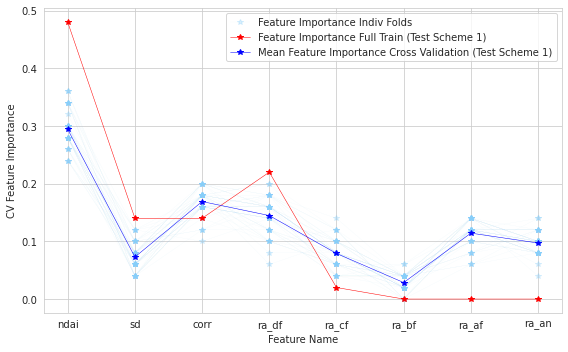
\includegraphics[width=0.48\textwidth]{statics/Feature_importance_test_scheme1_tr_12_te_3.png} }}
    \qquad
    \subfloat[\centering Histograms of NDAI (Left), Corr (Center), and SD (Right), between misclassified and correctly classified \textbf{Surface}(Non-Cloud) data points. \textcolor{blue}{Blue} histograms represent the distribution of features of points that are correctly classified and \textcolor{orange}{orange} those that are mis-classified]{{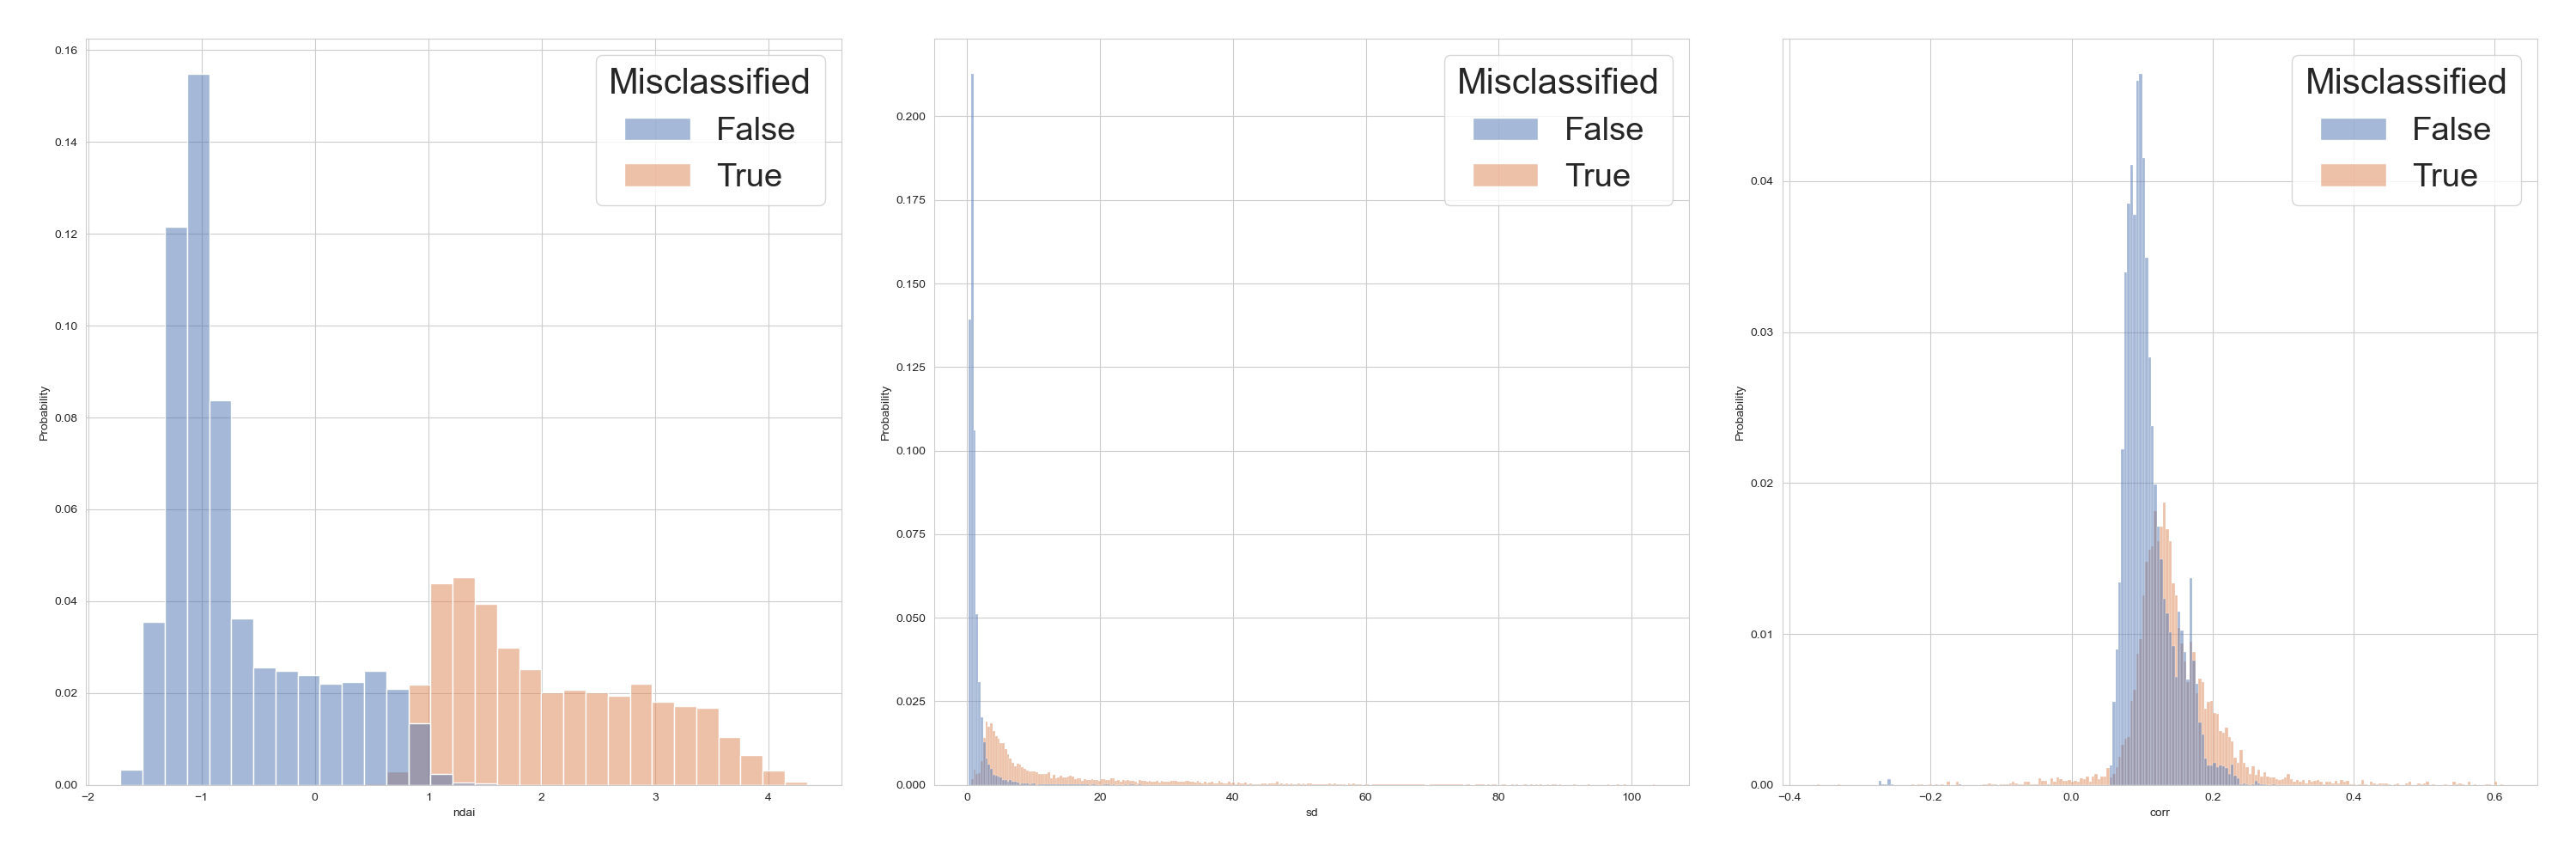
\includegraphics[width=0.48\textwidth]{statics/feature_compare_true_neg_tr_12_te_3.png} }}
    \qquad
    \subfloat[\centering Histograms of NDAI (Left), Corr (Center), and SD (Right), between misclassified and correctly classified \textbf{Cloud} data points. \textcolor{blue}{Blue} histograms represent the distribution of features of points that are correctly classified and \textcolor{orange}{orange} those that are mis-classified]{{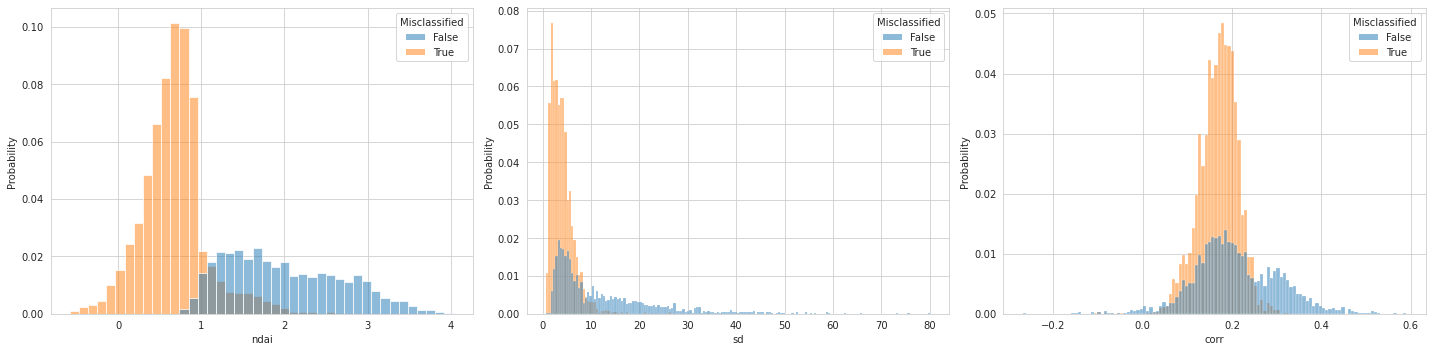
\includegraphics[width=0.48\textwidth]{feature_compare_true_pos_tr_12_te_3.png} }}
    \caption{Top: Feature Importance Under Alternative Splits. Middle: Feature value histograms for cloud-labeled pixels under alternative splits. Bottom:  Feature value histograms for surface labeled pixels under alternative splits }
    \label{fig:combined_feature_importance_and_hist}
\end{figure}

\subsubsection{Decision Surface}
Next, we analyze the decision surface of Adaboost. This is a similar analysis to that in the previous section, except that now instead of analyzing predicted probabilities concerning the spatial coordinates of the pixel, we do so for the features used. There are in total 8 features used, meaning that the decision surface cannot be easily visualized due to the high dimension. We thus conduct a PCA first, projecting the feature space into 2 dimensions. These learned PCA components are then used to inversely project a grid of 2 dimension points to the 8-dimensional feature space, which we can then classify using the model. By doing this, we can obtain a low-dimensional representation of the decision surface of our model. This is represented in Figure \ref{fig:decision_surface}. For comparison, we have also plotted the decision surface of the logistic regression model. Once again, we can see a similar trend as in Figure \ref{fig:Probability_Preds}. The model tends to be more confident in the non-cloud (blue) prediction versus the cloud (red) prediction. We further see a more complex decision surface where regions with mostly cloud points have high classification probability. As the space becomes mixed with cloud and non-cloud points, the confidence in classifying as non-clouds steadily decreases and shifts towards classifying as clouds as we move into the space populated mainly by cloud points. Interestingly, as we move further toward the top right of the 2D space, the model becomes less confident about its predictions. Contrast this to the decision surface generated by the logistic regression. In this case, the decision surface is almost uniformly confident throughout the two regions of its decision surface. It exhibits very high confidence in regions with little data or where there is a lot of overlapping data from both classes. Combining the decision surface and the pixel-wise probabilities in Figure \ref{fig:Probability_Preds}. We conclude that the Adaboost algorithm can learn sensible probabilities. This accurate quantification of uncertainty by the Adaboost algorithm is important given the small amount of data available in the problem. Further, we see that as more data is given, Adaboost becomes more confident in its prediction, meaning that it has enough capacity to learn even more complex decision surfaces given more data.

\subsubsection{Misclassfication Deep-dive}
Next, we analyze differences in feature value distribution between correctly vs wrongly classified points for both true negatives and true positive cases. We plot the feature distribution of the three expert-derived features, NDAI, Corr, and SD, which are also the features of highest feature importance as seen in Figure \ref{fig:Feature_importance ts1}. For these plots, we first separate points that are clouds from those that are not clouds, then color-code them by whether they are correctly or wrongly classified. The resulting plots are shown in Figure \ref{fig:feature_val_compare}.

Across both the cloud and non-cloud data points, we see that there is a significant difference in the distribution of NDAI values between the correctly classified and the misclassified data points. This is likely to be a significant explainer of the model's error since NDAI is also the most important feature in the AdaBoost model. For example, in the non-cloud case in Figure \ref{fig:feature_val_compare}, we see that the mean of the distribution of NDAI for the misclassified points is significantly higher than that of the non-misclassified points. Contrast this with the histograms of Corr in Figure \ref{fig:feature_val_compare}, where the distributions of the non-misclassified points and the misclassified points are indistinguishable if not for the labels. In this case, we can see that the model's heavy reliance on the NDAI feature might be one of the key drivers of error in the model.

\subsection{Alternative Classifiers}
There are two key issues with our model. Firstly, our model ignores spatial dependencies between pixels; secondly, it is a supervised learning model that requires expert labels to train. Several models can explicitly account for spatial dependencies in images. One example would be the convolutional neural network, which we could train to produce pixel-wise outputs of the cloud prediction based on the input features (stacked as an image). Another option that doesn't require expert labeling is the Ising / Potts model, which explicitly encodes the spatial dependencies via an undirected graph. These two models should perform better than our selected classifiers by directly modeling the innate spatial dependencies of the image data.

As we mentioned, our algorithm requires expert labels to train, which is often time-consuming and not easily obtainable. The main concern is the relatively small set of images we have for training. As such, we will likely encounter future test images of highly different covariate distributions (data drift) and also different covariate-to-output relations (concept drift). The currently trained classifier will perform poorly on these edge cases. As such, unless we have a bigger training dataset, we are not confident of the model's ability to generalize to a large set of new images.

\subsection{Stability with Alternative Training Splits}
To check the robustness of our conclusions about Adaboost in the earlier sections, we vary the images used for training and for testing. This time, we use images 1 and 2 for training and 3 for testing. This is a significant change due to the larger number of cloud-labeled data points in image 1. We then re-run the earlier analysis, plotting them in Figures \ref{fig:Probability_Preds_alt}, \ref{fig:decision_surface_alt} and \ref{fig:combined_feature_importance_and_hist}.

\subsubsection{Decision Surfaces}
Figure \ref{fig:decision_surface_alt} shows the learned decision surface with new training points overlaid with points from the test set. Once again, we see that, unlike logistic regression, Adaboost does not overfit on predicted probabilities, which can be seen by Adaboost learning a less confident decision surface, especially near boundaries and in areas with low data. 
\subsubsection{Predicted Probabilities}
We see a similar trend in predicted probabilities as before. The new predicted probabilities are shown in Figure \ref{fig:Probability_Preds_alt}. Once again, we see that the model tends to misclassify isolated patches, preferring to learn spatially homogenous patches; neighboring pixels tend to have the same prediction.
\subsubsection{Feature Values}
We see from Figure \ref{fig:combined_feature_importance_and_hist} that the main driver of misclassification is the differing distribution of NDAI. In fact, with the larger number of true positive (cloud) points in the training set, the differences in NDAI are even more apparent. 


\section{Conclusion}
In this report, we have conducted a thorough trial of several different machine learning based classifiers for the prediction of Arctic Clouds from MISR satellite images. The models we tested consist of expert labelled features used as input into various machine learning models. We have tested four models, the logistic regression, CART, Random Forest and Adaboost. We have implemented a rigorous model validation framework, using two different testing schemes that account for the non-IID nature of the pixels. Based on these testing schemes we have chosen Adaboost as the best model. We then conducted further analysis of Adaboost, which further reveals many interesting and beneficial properties of Adaboost. Firstly, we saw that Adaboost can learn well-calibrated decision surfaces, despite the relative lack of data. Secondly we saw that in Adaboost, feature importance are relatively stable across different cross validation folds and testing folds. These insights lead us to conclude that the Adaboost algorithm will perform well given a larger set of images. As such we conclude that expertly crafted features used in conjuction with Adaboost and trained on a large set of MISR image data will form the basis of a highly accurate cloud detection system.


\end{document}